\chapter{Available Modules and How to Use Them}
\label{ch:modules}
% ##################################################################################################################
% ##################################################################################################################

\hfill \textbf{Author:} Andreas Horni

\begin{center} 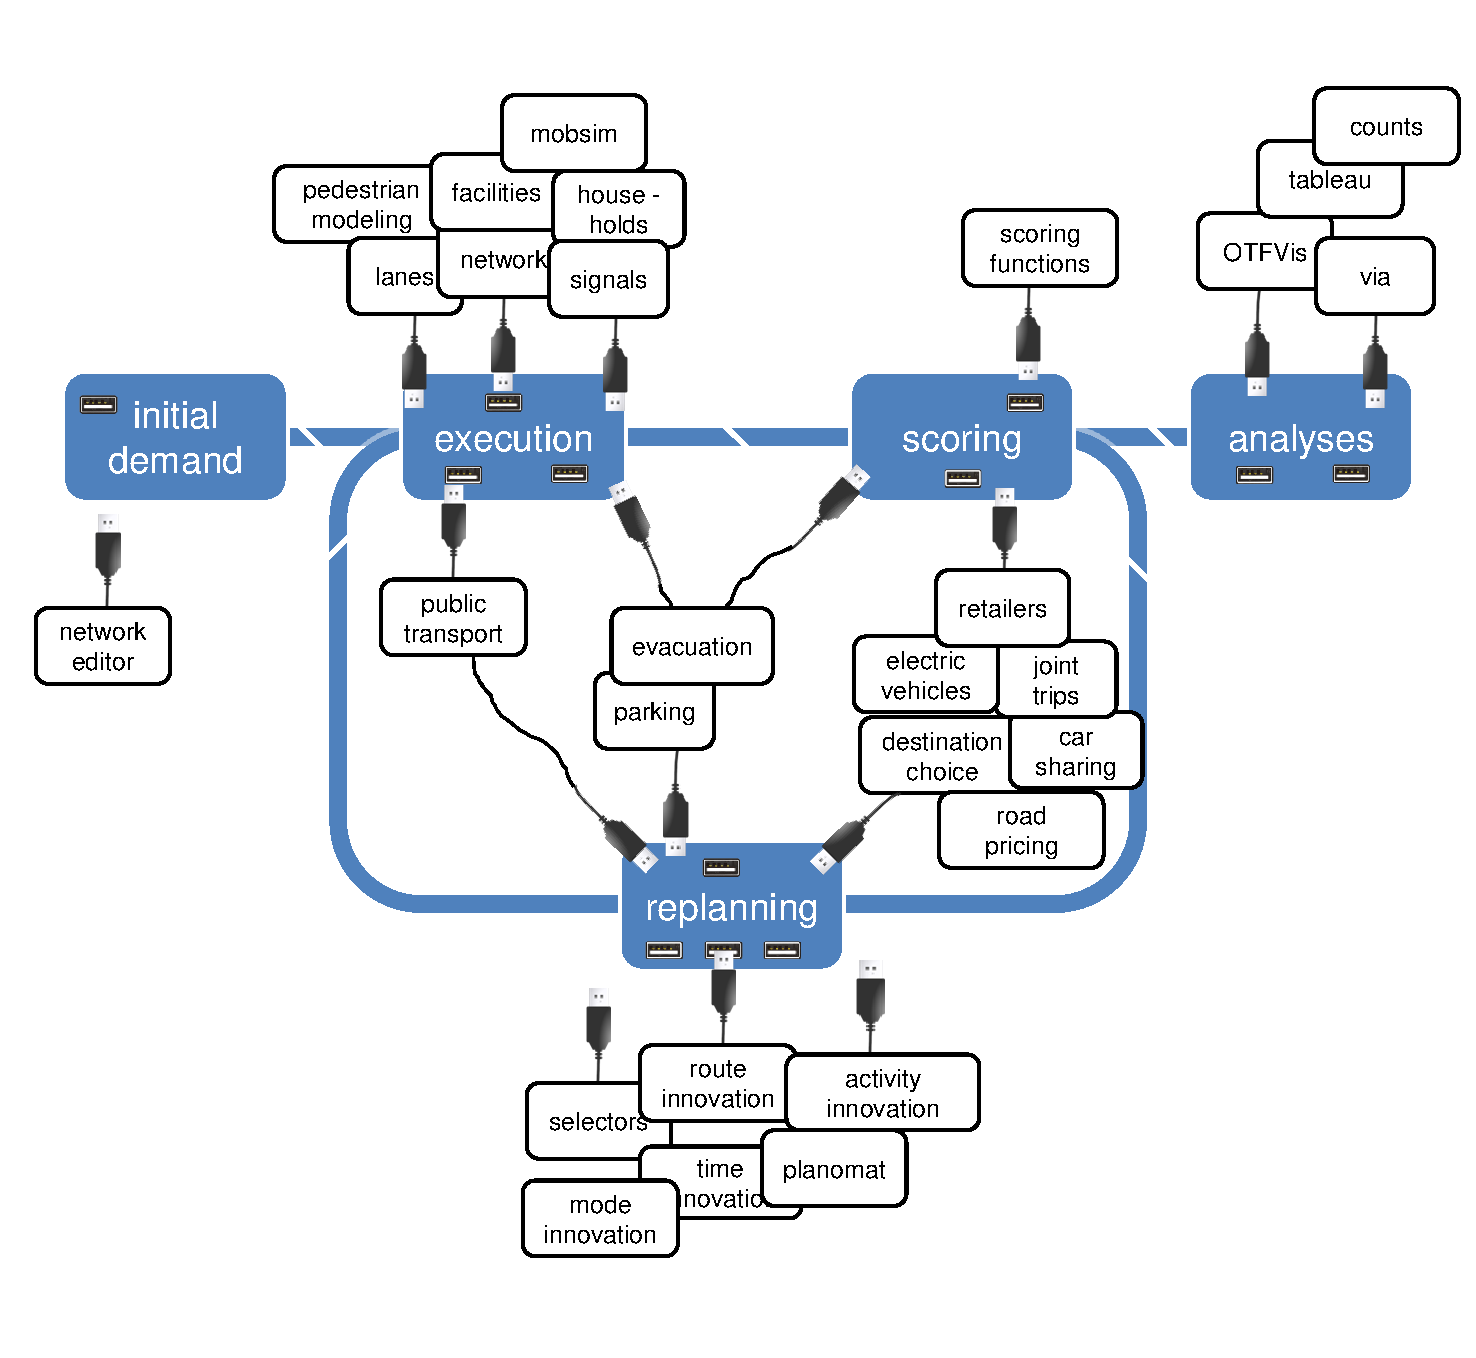
\includegraphics[width=0.5\textwidth, angle=0]{extending/figures/modules.pdf} \end{center}

% ##################################################################################################################
In this chapter you will learn about the possibilities to configure, extend, and customize MATSim by available functionality. In Chapter~\ref{ch:extensionpoints} you will see, how you can hook in your own extensions.

% ##################################################################################################################
\section{MATSim Modules}
The basic concept to extend MATSim is the usage of modules. But, please be aware that when it comes to configuring MATSim the term ``module'' is very extensively used such that a clear definition of what is a module and what is not is not available to date. This consequence of organic grows be corrected on the long run, for now, we try to just sort out the different meanings of the word module. 

Following different components are called modules.

\paragraph{Components in \lstinline|org.matsim|:} % --------------
The term ``module'' is used for components providing distinct functionality, residing in the \lstinline|org.matsim| package and having their own section in the default configuration file. Such a section looks as follows. 
\begin{lstlisting}
<module name="aModule"> 
    <param name="aParameterForAModule0" value="someValueX" /> 
    <param name="aParameterForAModule1" value="someValueY" />  
</module>
\end{lstlisting}

\paragraph{Contributions:} % --------------
The term ``module is furthermore used for contributions, residing in the \lstinline|org.matsim.contrib| package and either having their section in the default configuration file (such as destination choice) or not (such as the wagonsim contribution). 

\paragraph{External Functionality:} % --------------
Also external components plugged in and replacing a MATSim module, such as a mobsim, are called modules.

MATSim provides the possibility that the parameters of arbitrary external modules are added to the configuration file as shown above. In the respective module, the parameters can be accessed with the method \lstinline|public final String findParam(final String moduleName, final String paramName)| of the \lstinline|Config| class.

\paragraph{Standalone Tools:} % --------------
Also the standalone tools referencing MATSim as a library, such as the network editor, or the visualizer via, are termed modules in current practice.

\paragraph{Replanning Modules:} % --------------
A slightly different meaning of modules, which is only relevant for the MATSim developer and API-user, is as follows. In the package package \lstinline|org.matsim.core.replanning.modules| replanning functionality is provided in classes that are derived from \lstinline|AbstractMultithreadedModule|. 

% ===================================================================================
\subsection{Current Problems With Modules}
The majority of the replanning modules have their own section in the configuration file, but some do not, such as the \lstinline|TripsToLegsModule|. In that package---called modules---there are furthermore, the factories for the plan selectors. For the selectors and their factories, it is unclear if they are modules.

To make things worse, there are cases where module names in the configuration file are not (yet) consistent with the naming in the code. Examples are ``\lstinline|strategy|'' in the configuration file and ``\lstinline|StrategyManager|'' in the code, or ``strategy module'' in the config file and ``\lstinline|PlanStrategy|'' in the code \ah{Nochmals nachsehen!}. Furthermore, modules are atomic. There is, for example, a module called ``\lstinline|ChangeSingleLegMod|'', a module ``\lstinline|ChangeLegMode|'' and a module ``\lstinline|SubtourModeChoic|'' instead of one single module called ``\lstinline|ModeChoice|''. This, on the one hand, has historical reasons; the three modules were developed temporally separated. On the other hand, the parameter set for a module is only minimal and unambiguous if provided for atomic modules as different parameters are required for the three modules.

For the presentation of the available functionality, we chose to not use a single section per module but to group them according to common transport planning categories, in the example above this would be ``mode choice'' instead of the atomic categories, where we use terms ``functionality'' for the larger categories and ``module'' for the atomic components. 

Due to the distributed and project- and dissertation-driven MATSim contribution process (see Chapter \ref{ch:developmentprocess} modules are usually implemented for a specific practical purpose leading to various limitations of the respective module, e.g., modules might only work for a specific mode or for a defined calling order. Before, an additional effort is undertaken to generalize the module toward its embedding in the complete framework, the combination of a specific module with other functionality remains a non-straight-forward task. This means, that the user is in charge of systematically testing a specific modules combination before productively applying it.

% ##################################################################################################################
\section{An Overview of Existing Modules}
Figure~\ref{fig:matsimmodules} shows where in the MATSim loop, common MATSim modules can be plugged in. The technical details for their usage, in particular the parameter sets are described in \citep[][]{MATSim_Userguide_2014} and in the javadoc.
%
\createfigure%
{MATSim functionality}%
{MATSim functionality}%
{\label{fig:matsimmodules}}%
{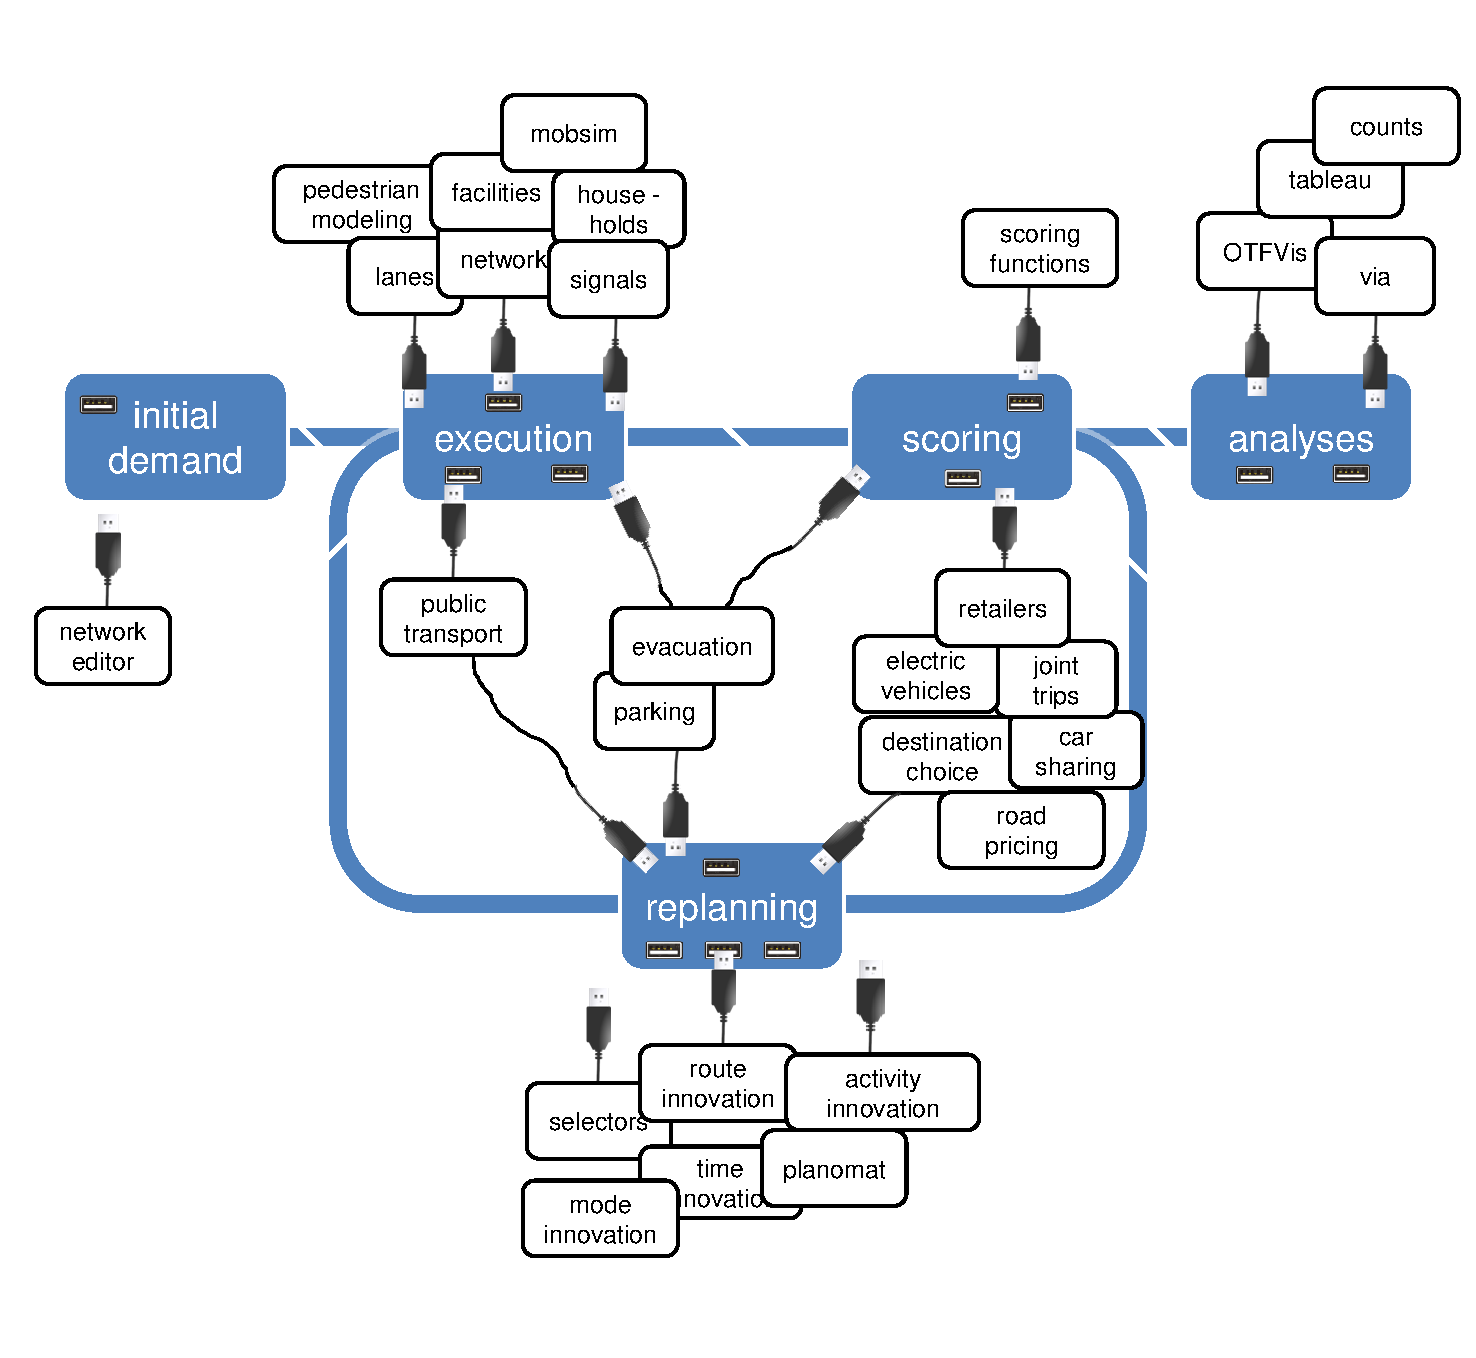
\includegraphics[width=0.99\textwidth, angle=0]{extending/figures/modules.pdf}}%
{}
%
The description of the modules in this and the following chapters is based on following categorization.
%
\createtable%
{Modules}%
{Modules}%
{\label{tab:modules}}%
{%
  \begin{tabular}[c]{|l|l|}
	\hline
	\textbf{Strategy Modules} & Section~\ref{sec:strategymodules} \\
	\hline
	Time Choice & Section~\ref{sec:timechoice} \\
	Route Choice & Section~\ref{sec:routechoice} \\
	Mode Choice & Section~\ref{sec:modechoice} \\
	Selectors & Section~\ref{sec:selectors} \\
	Destination Choice & Chapter~\ref{ch:destinationchoice} \\
	\hline
	\textbf{Further Choice Modules} & Section~\ref{sec:furtherchoicemodules} \\
	\hline
	Planomat & Section~\ref{sec:planomat} \\
	Activity Choice a.k.a. PlanomatX & Section~\ref{sec:activitychoice} \\
	Within-day Replanning & Chapter~\ref{ch:withinday} \\
	\hline
	\textbf{Supply-Side Modules} & Section~\ref{sec:supplysidemodules} \\
	\hline
	Network & Section~\ref{sec:network} \\
	Counts & Section~\ref{sec:counts} \\
	Facilities & Section~\ref{sec:facilities} \\
	Signals and Lanes & Chapter~\ref{ch:signalslanes} \\
	\hline
	\textbf{Demand-Side Modules and Specific Transport Modes Modules} & Section~\ref{sec:dsm} \\
	\hline
	Population & Section~\ref{sec:population} \\
	Households & Section~\ref{sec:households} \\
	Vehicles & Section~\ref{sec:vehicles} \\
%	Flight Traffic & Section~\ref{sec:flighttraffic} \\
	Public Transport & Chapter~\ref{ch:pt} \\
	Multi-Modal Simulation & Chapter~\ref{ch:multimodalsim} \\
	Freight Traffic & Chapter~\ref{ch:freight} \\
	Car Sharing & Chapter~\ref{ch:carsharing} \\
	Joint Trips and Social Networks & Chapter~\ref{ch:jointtrips} \\
	Dynamic Transport Systems & Chapter~\ref{ch:dts} \\
	Parking & Chapter~\ref{ch:parking} \\ 
	Electric Vehicles & Chapter~\ref{ch:elvehicles} \\
	\hline
	\textbf{Mobsims} & Section~\ref{sec:mobsims} \\
	\hline
	QSim & Section~\ref{sec:qsim} \\
	JDEQSim & Section~\ref{sec:jdeqsim} \\
	queueSimulation & Section~\ref{sec:queueSimulation} \\
	DEQSim & Section~\ref{sec:deqsim} \\
	\hline
	\end{tabular}
}%
{}
	
\createtable%
{Modules continued}%
{Modules continued}%
{\label{tab:modulescontinued}}%
{%
  \begin{tabular}[c]{|l|l|}
	\hline
	\textbf{General Purpose Modules} & Section\ref{sec:generalpurposemodules} \\
	\hline
	Controler & Section~\ref{sec:controler} \\
	Global & Section~\ref{sec:global} \\
	Scenario & Section~\ref{sec:scenario} \\
	Scoring & Section~\ref{sec:scoring} \\ 
	\hline	
	\textbf{Special Purpose Modules, Tools and Functionalities} & Section~\ref{sec:specialpurpose} \\
	\hline
	Travel Time Calculator & Section~\ref{sec:ttc} \\
	Link Stats & Section~\ref{sec:linkStats} \\
	OTFVis Visualizer & Section~\ref{sec:OTFVis} \\
	Senozon via Visualizer & Section~\ref{sec:via} \\
	Cadyts & Section~\ref{sec:cadyts} \\
	Landuse & Section~\ref{sec:landuse} \\
	Parallel Computing & Section~\ref{sec:parallelcomputing} \\
%	Extension of Simulation Horizon & Section~\ref{sec:longitudinalscenario} \\
%	Warmstart & Section~\ref{sec:warmstart} \\
	Roadpricing & Chapter~\ref{ch:roadpricing} \\
	Emisssions & Chapter~\ref{ch:emissions} \\
	Accessibility & Chapter~\ref{ch:accessibility} \\
	Evacuation & Chapter~\ref{ch:evacuation}  \\
	WagonSim & Chapter~\ref{ch:wagonSim} \\
	PSim & Chapter~\ref{ch:psim} \\
	Network editors &  Chapter~\ref{ch:networkeditor} \\
	Business Analytics & Chapter~\ref{ch:businessanalytics} \\
	\hline
	\end{tabular}
}%
{}

% ##################################################################################################################
\section{Strategy Modules}
\label{sec:strategymodules}
The strategy modules are the basic choice modules available in MATSim. All strategy modules are called by configuring the strategy module in the configuration file as shown in the following example.

\begin{lstlisting}
<module name="strategy" > 
    <param name="ModuleProbability_1" value="0.1" /> 
    <param name="Module_1" value="ChangeLegMode" /> 
    <param name="ModuleProbability_2" value="0.2" /> 
    <param name="Module_2" value="TimeAllocationMutator" /> 
    <param name="ModuleProbability_3" value="0.7" /> 
    <param name="Module_3" value="SelectExpBeta" /> 
</module>
\end{lstlisting}

Strategy modules are numbered, where each module is given a weight which determines the probability by which the course of action represented by the module is taken. In this example, each agent changes his leg mode with probability 0.1, its plan timing with probability 0.2. A strategy module is, in the code, always a combination of a plan selector and zero or more strategy module elements. In the example, the agent choses a plan from his set of plans according to a logit model with probability 0.7. The weights of the strategy modules are renormalized in case they do not sum to one. 

Combining different modules is not straight-forward in MATSim. This important topic urgently awaits future analysis. To begin with, here, the combination of the strategy modules with public transport is presented in Table \ref{tab:combination}.

% ----------------------------------
\createtable%
{Strategy Module Combination}%
{Strategy Module Combination}%
{\label{tab:combination}}%
{%
  \begin{tabular}[c]{|c|c|c|}
   \hline
\textbf{Choice Dimension}	& \textbf{Default Strategy} & \textbf{Public Transport}\\
\hline
time choice & TimeAllocationMutator &  TransitTimeAllocationMutator\\
\hline
route choice & ReRoute & ReRoute \\
\hline
mode choice & \multirow{2}{*}{ChangeLegMode} & \multirow{2}{*}{TransitChangeLegMode} \\
(all legs get same mode) &  &  \\
\hline
mode choice & \multirow{2}{*}{ChangeSingleLegMode} & \multirow{2}{*}{TransitChangeSingleLegMode} \\
(each leg can have a different mode) &  &  \\
\hline
mode choice & \multirow{2}{*}{SubtourModeChoice} & \multirow{2}{*}{TransitSubtourModeChoice} \\
(subtour-based) &  &  \\
\hline
destination choice & LocationChoice & LocationChoice \\
\hline
  \end{tabular}
}%
{}

% ===================================================================================
\subsection{Time Choice}
\label{sec:timechoice}
\begin{compactitem}
\item Invoking the module: Time choice is applied by defining its parameters in the configuration file and by adapting the configuration file strategy module as follows 
%
\begin{lstlisting}
<module name="strategy" > 
    <param name="ModuleProbability_1" value="0.x" /> 
    <param name="Module_1" value="TimeAllocationMutator" /> 
    [...]
</module>
\end{lstlisting}
%
\item Configuration: \lstinline|TimeAllocationMutator| config file section
\item Code: \lstinline|org.matsim.core.replanning.modules.TimeAllocationMutator|
\end{compactitem}

The module shifts activity end times randomly within a configurable range as described by \citet[][]{BalmerEtAl_Timmermans_2005, Raney_PhDThesis_2005, Balmer_unpub_VSP_2004, BalmerEtAl_unpub_EIRASS_2004, BalmerEtAl_unpub_STRC_2004}. A best-reponse approach to time choice is applied by ``planomat'' described in Section \ref{sec:planomat}.

% ===================================================================================
\subsection{Route Choice} 
\label{sec:routechoice}
\begin{compactitem}
\item Invoking the module: Route choice is applied by defining its parameters in the configuration file and by adapting the configuration file strategy module as follows
%
\begin{lstlisting}
<module name="strategy" > 
    <param name="ModuleProbability_1" value="0.x" /> 
    <param name="Module_1" value="ReRoute" /> 
    [...]
</module>
\end{lstlisting}
%
\item Configuration: \lstinline|planscalcroute| config file section. The routing algorithm needs to be specified in the configuration file controler module 
%
\begin{lstlisting}
<module name="controler" > 
    <param name="routingAlgorithmType" value="{Dijkstra | FastDijkstra | 
    		AStarLandmarks | FastAStarLandmarks}" /> 
    [...]
</module>
\end{lstlisting}
\item Code: \lstinline|org.matsim.core.router|
\end{compactitem}

MATSim routing is described by \citet[]{LefebvreBalmer_STRC_2007, LefebvreBalmer_TechRep_IVT_2007}. The configuration necessary for public transport is shown in Chapter \ref{ch:pt}.

% ===================================================================================
\subsection{Mode Choice}
\label{sec:modechoice}
\begin{compactitem}
\item Invoking the module: Mode choice is applied by defining its parameters in the configuration file and by adapting the configuration file strategy module by choosing one of the mode choice options as follows
\begin{lstlisting}
<module name="strategy" > 
    <param name="ModuleProbability_1" value="0.x" /> 
    <param name="Module_1" value="{ChangeLegMode | 
    		ChangeSingleLegMode | SubtourModeChoice}" /> 
    [...]
</module>
\end{lstlisting}
%
\item Configuration: Corresponding with the chose type of mode choice a respective config file section needs to be added:
%
\begin{lstlisting}
<module name="{changeLegMode | 
				changeLegMode | subtourModeChoice}" > 
    <param name="param0" value="value0" /> 
    [...]
</module>
\end{lstlisting}
%
\item Code: \lstinline|org.matsim.core.replanning.modules| and \lstinline|org.matsim.population.algorithms|.
\end{compactitem}

\lstinline|ChangeLegMode| randomly picks one of the plans of a person and changes its mode of transport. By default, the supported modes are driving a car and using public transport. Only one mode of transport per plan is supported. For using different modes for sub-tours on a single day the \lstinline|SubtourModeChoice| module is required. Optionally, car-availability is respected. \lstinline| ChangeSingleLegMode| randomly picks one of the plans of a person and changes the mode of transport of one single leg. The leg is picked randomly. In contrast to \lstinline|ChangeLegMode|, it allows for multiple modes in one plan. By default, the supported modes are driving a car and using public transport. Also, this module is able to (optionally) respect car-availability. 
 
Mode choice is described by \citet[][]{RieserEtAl_TRR_2009, MeisterEtAl_WCTRS_2010, CiariEtAl_STRC_2008, CiariEtAl_STRC_2007}.

% ===================================================================================
\subsection{Selectors}
\label{sec:selectors}
\begin{compactitem}
\item Invoking the module: Define one of the available selectors in the configuration file strategy module as follows
%
\begin{lstlisting}
<module name="strategy" > 
    <param name="ModuleProbability_1" value="0.x" /> 
    <param name="Module_1" value="{a specific selector}" /> 
    [...]
</module>
\end{lstlisting}
%
Following selectors are available in the configuration file strategy module: 
%
\begin{compactitem}
	\item \lstinline|KeepLastSelected| keeps the plan selected in the previous iteration.
	\item \lstinline|BestScore| selects the plan with the highest score of the previous iteration.
	\item \lstinline|SelectExpBeta| performs multinomial logit model selection between plans.
	\item \lstinline|ChangeExpBeta| changes to a different plan with probability dependent on $e^{\Delta_{score}}$, where $\Delta_{score}$ is the score difference between the two plans. 
	\item \lstinline|SelectRandom| performs random selection between the plans.
	\item \lstinline|SelectPathSizeLogit| selects an existing Plan according to the Path Size Logit described by \citet[][]{FrejingerBierlaire_TransResB_2007}.
\end{compactitem}
% 
\item Configuration: no further configuration necessary \ah{? selectExpBeta ...}
\item Code: \lstinline|org.matsim.core.replanning.selectors| 
\end{compactitem}

Note, that the \lstinline|BestScore| should be used with care as it is prone to getting stuck with sub-optimal plans. Plans that are rated bad due to a random fluctuation in one single iteration, due to e.g., a rare traffic jam, will never be tested again. It is therefore recommended to use this in conjunction with \lstinline|SelectRandom| only.

Besides the selectors for plan modification and execution, in the near future also the plan remover will be available for configuration. Per default, the plan with the lowest score is removed if the agent's memory is full. In line with the requirements of e.g., simulated annealing approaches, the removal of candidates will be configurable to be probabilistically dependent on the plan score similar to the selection in \lstinline|SelectExpBeta|. This will reduce the probability to get stuck with sub-optimal plans, that were dominant in earlier iterations.
\ah{siehe Mail by M. Zilske, August 14 ``[Matsim-devel] custom plan selector for removal'')}

% ##################################################################################################################
\section{Further Choice Modules}
\label{sec:furtherchoicemodules}
% ===================================================================================
\subsection{Planomat}
\label{sec:planomat}
\begin{compactitem}
\item Invoking the module: The Planomat module cannot be invoked directly anymore; it is not available in current releases anymore but can be downloaded from SVN history. \ah{�hm, stimmt das?}
\item Configuration: see above
\item Code: see above
\end{compactitem}

A special replanning module using a different logic than undirected trial-and-error was Planomat. Planomat did not evaluate just one random alternative per iteration but multiple alternatives within one single iteration to obtain a (at least locally) optimal solution. It used a genetic algorithm \citep[][]{MeisterEtAl_IATBR_2006, MeisterEtAl_STRC_2006, Meister_PhDThesis_2011} for this purpose. Planomat was successfully applied in the project \emph{KTI Frequencies} for time choice and mode choice for sub-tours \citep[][p.10]{BalmerEtAl_ResRep_datapuls_2010}. 

% ===================================================================================
\subsection{Activity Choice a.k.a. PlanomatX}
\label{sec:activitychoice}
\begin{compactitem}
\item Invoking the module: The PlanomatX module cannot be invoked directly anymore; it is not available in current releases anymore but can be downloaded from SVN history.
\item Configuration: see above
\item Code: see above
\end{compactitem}

PlanomatX performing activity choice and adopting a Tabu Search approach is described by \citet[][]{Feil_PhDThesis_2010}. To cope with curse of dimensionality due to the added choice dimension, PlanomatX introduced schedule recycling, which is basically a warmstart concept. Due to the problems with a logarithmic utility function for activity choice as reported in Section \ref{sec:utfextensions}, PlanomatX furthermore replaced to standard MATSim scoring function by an S-shaped one. Rough estimates for its parameters based on an multinomial logit model (MNL) exist.

% ===================================================================================
% ##################################################################################################################
\section{Supply-Side Modules}
\label{sec:supplysidemodules}

% ===================================================================================
\subsection{Network}
\label{sec:network}
\begin{compactitem}
\item Invoking the module: By adding the respective configuration file section, the module is invoked automatically.
\item Configuring: \lstinline|network| config file section
\item Code: \lstinline|org.matsim.core.network|
\end{compactitem}

It is possible to make network attributes time-dependent, as observed in reality in case of accidents or adaptive traffic control, with varying speed limits or driving directions of lanes on multi-lane roads with heavily unbalanced load over the course of a day. Attributes that can be adapted are free speed, number of lanes and flow capacity. 

The adaptation can be specified by adding following two lines to the \lstinline|network| configuration file section:
\begin{lstlisting}
<param name="timeVariantNetwork" value="true" />
<param name="inputChangeEventsFile" value="path_to_change_events_file" /> 
\end{lstlisting}
% 
An example file setting the free speed of three network links to zero is as follows:
%
\begin{lstlisting}
<?xml version="1.0" encoding="UTF-8"?> 
	<networkChangeEvents xmlns="http://www.matsim.org/files/dtd"  
	xmlns:xsi="http://www.w3.org/2001/XMLSchema-instance"  
	xsi:schemaLocation="http://www.matsim.org/files/dtd  
	http://www.matsim.org/files/dtd/networkChangeEvents.xsd">} 
 
  <networkChangeEvent startTime="03:06:00"> 
    <link refId="12487"/> 
    <link refId="12489"/> 
    <link refId="12491"/> 
    <freespeed type="absolute" value="0.0"/> 
  </networkChangeEvent> 
 
</networkChangeEvents> 
\end{lstlisting}
% 
Alternatively, network change events can be directly added to the code as follows:
\begin{lstlisting}
networkChangeEvent = 
	network.getFactory().createNetworkChangeEvent(...);
networkChangeEvent.setFlowCapacityChange(new ChangeValue(...));
networkChangeEvent.setFreespeedChange(new ChangeValue(...));
networkChangeEvent0.setLanesChange(new ChangeValue(...));
network.addNetworkChangeEvent(networkChangeEvent);
\end{lstlisting}

% ===================================================================================
\subsection{Counts}
\label{sec:counts}
\begin{compactitem}
\item Invoking the module: By adding the respective configuration file section, the module is invoked automatically.
\item Configuration: \lstinline|counts| file section  
\item Code: \lstinline|org.matsim.counts| 
\end{compactitem}

MATSim offers the possibility to perform link volume comparisons between simulated and counted value for both motorized individual traffic \citep{Horni_unpub_IVT_2007}  and public transport. The later are described in Chapter \ref{ch:pt}. The count package offers analyses for the average working day with hourly resolution. A google maps based visualization is available, showing each station with a its load curve in a pop-up window at the geographic location.

As shown by \citet[][]{BalmerEtAl_ResRep_bdktzrh_2009}, for the Z�rich scenario link volume comparisons have been successfully performed with data based on city level, cantonal level and national level \citep[][]{ASTRA_Webpage_2006}, where an average working day (Monday to Thursday, excluding public holidays) was built. Usually it is helpful to exclude a substantial part of the outer range of the modeled study region to prevent boundary effects.

% ===================================================================================
\subsection{Facilities}
\label{sec:facilities}
\begin{compactitem}
\item Invoking the module: By adding the respective configuration file section, the module is invoked automatically. Please make sure, that added modules can manage facilities.
\item Configuration: \lstinline|facilities| configuration file section
\item Code: \lstinline|org.matsim.core.facilities|
\end{compactitem}

Facilities are a non-mandatory element of MATSim scenarios. They identify activity locations and can hold opening hour and capacity information. facilities are mostly used in the MATSim Z�rich group, in particular in the Z�rich scenario, where facilities are derived from the Federal Enterprise Census 2001 \citep[][]{SwissEnterpriseCensus_manual_2001} providing hectare level information and using NOGA-classification. Detailed technical description of facilities generation is given by \citet[][]{Meister_TechRep_IVT_2008, Meister_unpub_IVT_2007}. 

% ===================================================================================

% ##################################################################################################################
\section{Demand-Side Modules and Specific Transport Modes Modules}
\label{sec:dsm}

% ===================================================================================
\subsection{Population}
\label{sec:population}
\begin{compactitem}
\item Invoking the module: By adding the respective configuration file section, the module is invoked automatically.
\item Configuration: \lstinline|plans| config file section. Optionally the path to a person attributes file in \lstinline|ObjectAttributes| format can be specified.
\item Code: \lstinline|org.matsim.core.population|
\end{compactitem}

The population module manages transport demand, i.e., the population and the agents' plans.
% ===================================================================================
\subsection{Households}
\label{sec:households}
\begin{compactitem}
\item Invoking the module: Enable househlds in the \lstinline|scenario| section of the configuration file and provide the paths to a households file and another file containing the households' attributes in the configuration file section \lstinline|households|.
\item Configuration: \lstinline|households| config file section
\item Code: \lstinline|org.matsim.households|
\end{compactitem}

Similar to the vehicles module, the household module is not used by default in MATSim.

% ===================================================================================
\subsection{Vehicles}
\label{sec:vehicles}
\begin{compactitem}
\item Invoking the module: Vehicles need to be enabled in the \lstinline|scenario| configuration file section.
\item Configuration: At the moment vehicles are only used for public transport (Chapter \ref{ch:pt}), i.e., motorized individual traffic vehicles are not used in MATSim nowadays. Thus, the configuration file section specifying the input file is located in the \lstinline|transit| configuration file section, while the vehicles module does not have its own configuration file section. \ah{Kl�ren, ob man diese kleine Inkonsistenz beheben m�chte.} This might change one day when the parking module will start to use vehicles. \citet[][]{JaeggiEtAl_TRR_2012} might serve as an empirical base for the assignment of vehicles to agents or households.
\item Code: \lstinline|org.matsim.vehicles|
\end{compactitem}

The vehicles package provides a file reader and a factory to create vehicles. 

% ===================================================================================
%\subsection{Flight Traffic}
%\label{sec:flighttraffic}
%Flight traffic is described by \citet[][]{Grether_PhDThesis_2014}.

% ===================================================================================

% ##################################################################################################################
\section{Mobsims}
\label{sec:mobsims}
An overview of MATSim mobility simulations is given in \citet[][]{Dobler_TechRep_IVT_2011}. See also the presentation of \citet[][]{Rieser_unpub_IVT_2011}.

% ===================================================================================
\subsection{QSim}
\label{sec:qsim}
\begin{compactitem}
\item Invoking the module: Set the parameter \lstinline|mobsim| of \lstinline|controler| config file section to \lstinline|qsim| provide a \lstinline|qsim| config file section. 
\item Configuration: \lstinline|qsim| config section
\item Code: \lstinline|org.matsim.core.mobsim.qsim|
\end{compactitem}

At the moment, in most applications \emph{QSim} \citep[][]{Dobler_TechRep_IVT_2011, Dobler_STRC_2010} is used. It has started as a software branch of \emph{queueSimulation} before supplanting this later simulation. Through multiple engines it can be run in parallel and simulate multi-modal traffic (Chapter~\ref{ch:multimodalsim}). It is queue-based and time-step based. The simulation is able to handle time-variant networks, within-day replanning \citep[][]{Dobler_TechRep_IVT_2009}, public transport \citep[][]{Rieser_PhDThesis_2010} and in an experimental manner also traffic lights \citep[][]{Neumann_MastersThesis_2008}). Inclusion of public transport is described in Chapter~\ref{ch:pt}.  

% ===================================================================================
\subsection{JDEQSim}
\label{sec:jdeqsim}
\begin{compactitem}
\item Invoking the module: Set the parameter \lstinline|mobsim| of \lstinline|controler| config file section to \lstinline|JDEQSim| provide a \lstinline|jdeqsim| config file section.
\item Configuration: \lstinline|jdeqsim| config file section
\item Code: \lstinline|org.matsim.core.mobsim.jdeqsim|
\end{compactitem}

\emph{JDEQSim} \citep[][]{WaraichEtAl_TechRep_IVT_2009, WaraichEtAl_STRC_2009} was used for project \emph{KTI Frequencies} \citep[][]{BalmerEtAl_ResRep_datapuls_2010}. It is is a java reimplementation of \emph{DEQSim} shown below \citep[][]{WaraichEtAl_STRC_2009, CharyparEtAl_TRR_2007, CharyparEtAl_TRB_2009} and provides parallel event handling but no parallel simulation \citep[][p.11]{BalmerEtAl_ResRep_datapuls_2010}. Back-propagating gaps, traffic lights, public transport and within-day replanning are not supported. Advice for \emph{JDEQSim} configuration can be found at (\ref{m:jdeqsim}).

% ===================================================================================
\subsection{queueSimulation (deprecated)}
\label{sec:queueSimulation}
The queueSim cannot be invoked directly anymore; it is not available in current releases anymore but can be downloaded from SVN history. The \lstinline|simulation| config file section is deprecated as well. \ah{stimmt das so?})

% ===================================================================================
\subsection{DEQSim (deprecated)}
\label{sec:deqsim}
\emph{DEQSim} was used for project \emph{Westumfahrung} \citep[][]{BalmerEtAl_ResRep_bdktzrh_2009}. It is a is a queue-based, event-based parallel simulation written in C++ \citep[][]{CharyparEtAl_TRR_2007, Charypar_PhDThesis_2008}. This simulation includes handling of reduced capacities due to traffic lights in an aggregate manner \citep[][p.139 ff]{Charypar_PhDThesis_2008}. It further supports modeling of gap back propagation at junctions \citep[][p.98 ff]{Charypar_PhDThesis_2008}. Events handling is done via file input and output. This represents a major bottleneck in terms of framework performance. Development of this simulation has been stopped and been replaced by the JAVA mobsim \emph{JDEQSim}.

% ===================================================================================
% ##################################################################################################################
\section{General Purpose Modules}
\label{sec:generalpurposemodules}

% ===================================================================================
\subsection{Controler}
\label{sec:controler}
\begin{compactitem}
\item Invoking the module: Run \lstinline|org.matsim.run.Controler|
\item Configuration: \lstinline|controler| configuration file section
\item Code: \lstinline|org.matsim.core.controler|
\end{compactitem}

The controler is an indispensable module for running MATSim. The module, can be furthermore extended by \lstinline|Events| and \lstinline|Listeners| as detailed in Chapter~\ref{ch:extensionpoints}. Classes implementing one or more \lstinline|Listener Interfaces| and can be registered with the Controler with \lstinline|addControlerListener()|. The controler fires \lstinline|Controler Events| at specific points during the run to the registered \lstinline|Listeners|, which can then execute their own code.

Another possibility to customize the controler is by inheritence from the class \lstinline|org.matsim.core.controler|.

% ===================================================================================
\subsection{Global}
\label{sec:global}
\begin{compactitem}
\item Invoking the module: The module is very sparse and only used to transfer some parameters to the simulation. Add a respective config file section.
\item Configuration: \lstinline|global| config file section. Arguably, this section should be merged with the controler section.
\item Code: \lstinline|org.matsim.core.config.groups.GlobalConfigGroup|
\end{compactitem}

The replanning modules get their information about number of threads from this module.

% ===================================================================================
\subsection{Scenario}
\label{sec:scenario}
\begin{compactitem}
\item Invoking the module: Add the respective config file section.
\item Configuration: \lstinline|scenario| config file section \ah{Hier haben wir doch eine kleine Inkonsistenz zwischen Container und Configuration Section, oder?}
\item Code: \lstinline|org.matsim.core.scenario|
\end{compactitem}

The \lstinline|scenario| module is, on the one hand, a container containing the main components of a scenario such as the \lstinline|config|, the \lstinline|network|, the \lstinline|population|, the \lstinline|facilities|, the \lstinline|transitSchedule|, \lstinline|households| and \lstinline|vehicles|. 

The config file section is, on the other hand, used in a slightly different manner. It defines the usage of lanes, signal systems, road pricing, agent knowledges, vehicles, households and public transport. Still a respective config file section is required for every additional functionality.

% ===================================================================================
\subsection{Scoring}
\label{sec:scoring}
\begin{compactitem}
\item Invoking the module: add below section to config file
\item Configuration: \lstinline|planCalcScore| config file section
\item Code: \lstinline|org.matsim.core.scoring|
\end{compactitem}

The parameters related to scoring described in Chapter \ref{ch:scoring}.

% ===================================================================================

% ##################################################################################################################
\section{Special Purpose Modules, Tools and Functionalities}
\label{sec:specialpurpose}

% ===================================================================================
\subsection{Travel Time Calculator}
\label{sec:ttc}
\begin{compactitem}
\item Invoking the module: The module is invoked by specifying the respective configuration file section.
\item Configuration: \lstinline|travelTimeCalculator| config file section
\item Code: \lstinline|org.matsim.core.trafficmonitoring|
\end{compactitem}

The routing module, as an example, needs travel time estimations for all links of the network. To keep the computational effort feasible, the travel time estimations need to aggregated to time bins. The parameters of this aggregation, such as the bin size, can be specified in the configuration file section \lstinline|travelTimeCalculator|. 

% ===================================================================================
\subsection{Link Stats}
\label{sec:linkStats}
\begin{compactitem}
\item Invoking the module: The module is invoked by specifying the respective configuration file section.
\item Configuration: \lstinline|linkStats| configuration file section
\item Code: \lstinline|org.matsim.analysis.CalcLinkStats|
\end{compactitem}

Link stats allow to specify the output interval of simulation statistics of individual links. They are amongst other, used for the comparison with count values. It is configurable, if the simulated volumes should be written per iteration or averaged over multiple iterations.

% ===================================================================================
\subsection{OTFVis Visualizer}
\label{sec:OTFVis}
\begin{compactitem}
\item Invoking the module: run \lstinline|org.matsim.contrib.otfvis.OTFVis|
\item Configuration: \lstinline|otfvis| configuration file section
\item Code: \lstinline|org.matsim.contrib.otfvis|
\end{compactitem}

Before senozon via the OTFVis (on-the-fly visualizer) \citep[][]{Strippgen_PhDThesis_2009} was the main visualization tool of MATSim. OTFVis is able to visualize results during runtime of a MATSim run. It is available as a contribution.

It is implemented in java, however, to make use of sophisticated visualization of the OpenGL framework, it is also heavily based on jogl. This requires a couple of user actions to get jogl running on his specific platform. This platform dependency has lead to some issue with the programs stability. It is thus recommended to use the senozon via. visualizer.

% ---------------------------
\subsection{Senozon via Visualizer}
\label{sec:via}
\begin{compactitem}
\item Invoking the module: via is a standalone visualizer
\item Configuration: separate configuration file
\item Code: proprietary
\end{compactitem}

Senozon via is the new and powerful MATSim visualizer. It is proprietary and can be bought from \citep[][]{senozonVIA_Webpage_2014}. Research licenses and a trial version are available. via is written in JAVA and distributed as a jar file. It offers various features such as dynamic visualization of vehicles and agents' activities, extensive analysis and query functionality and powerful plugins such as a movie maker or a car count data analyzer.

% ===================================================================================
\subsection{Cadyts}
\label{sec:cadyts}
\begin{compactitem}
\item Invoking the module: invoke \lstinline|CadytsContext| or \lstinline|CadytsPtContext|. Additionally activate pt or car counts. \ah{package info veraltet?}
\item Configuration: \lstinline|cadytsCar| or \lstinline|cadytsPt| config file section
\item Code: \lstinline|org.matsim.contrib.cadyts|
\end{compactitem}

Cadyts \citep[][]{FloetteroedEtAl_TechRep_TRANSPOR_2008} is a calibration tool that adjusts MATSim plans such that a measured calibration target is meet. Often count data is used as empirical data source.

% ===================================================================================
\subsection{Landuse}
\label{sec:landuse}
\begin{compactitem}
\item Invoking the module: run \lstinline|MATSim4UrbanSimZone| or \lstinline|MATSim4UrbanSimParcel| and provide a MATSim4Urbansim config file containing following two sections
\item Configuration: \lstinline|urbansimParameter| and \lstinline|matsim4urbansimControler| provided in a separate config file
\item Code: \lstinline|org.matsim.contrib.matsim4urbansim|
\end{compactitem}

The coupling of MATSim with UrbanSim \citep[][]{Waddell_unpub_UrbanSimTutorial_2010} is described in \citet[][]{NicolaiEtAl_TechRep_VSP_2011,NicolaiEtAl_ERSA_2011}.

% ===================================================================================
\subsection{Parallel Computing}
\label{sec:parallelcomputing}
\begin{compactitem}
\item Invoking the module: Define the number of threads in the \lstinline|qsim| and the \lstinline|parallelEventHandling| section
\item Configuration: \lstinline|parallelEventHandling| and \lstinline|qsim| configuration file section
\item Code: mainly \lstinline|org.matsim.core.events.ParallelEventsManagerImpl| for parallel event handling. See qsim for parallel mobsim running.
\end{compactitem}

As described in \citet[][]{WaraichEtAl_TechRep_IVT_2009, WaraichEtAl_STRC_2009} the simulation can be substantially speed-up when using multiple threads for the events handling, usually being a bottleneck in MATSim simulation runs. Amongst others, in the \lstinline|parallelEventHandling| configuration file section, the number of threads to be used can be specified. Clearly, the number of threads should correspond with available processor cores. As mentioned above, the mobsim \emph{QSim} is running parallel by default.

Being able to speed-up scenarios migth become even more important than today, when additional choice dimensions are added with large variability in the parameters rendering ensemble runs necessary (see Section~\ref{sec:variability}).

\ah{auch Doblers Arbeiten einf�gen!?}

\ah{Marcel hatte mal Testreihe mit Identifikation der Laufzeit einzelner Module (QSim, Eventshandling etc.) geplant. Nachfragen, ob schon was vorhanden}

% ===================================================================================
%\subsection{Extension of Simulation Horizon}
%\label{sec:longitudinalscenario}
%\begin{compactitem}
%\item Invoking the module:
%\item Configuration:
%\item Code:
%\end{compactitem}
%
%\who{Horni Surprice, Max/Fabian, Ordonez}
%Longitudinal Scenario \who{M�rki}
%
%\citep[e.g.,][]{HorniEtAl_TechRep_IVT_2012_a}.
%
%% ===================================================================================
%\subsection{Warmstarting}
%\label{sec:warmstart}
%\begin{compactitem}
%\item Invoking the module:
%\item Configuration:
%\item Code:
%\end{compactitem}
%
%\who{Horni Surpice, Dobler}

% ===================================================================================

% ##################################################################################################################
